\documentclass[12pt]{article}

\usepackage[english]{babel}
\usepackage[utf8]{inputenc}
\usepackage{amsmath}
\usepackage{graphicx}
\usepackage{amsfonts}
\usepackage[colorinlistoftodos]{todonotes}

\graphicspath{ {images/} }

\title{CS 5876 - HW 3}

\author{Joshua Campbell (jac677) , Michael Wang (mzw4) , Neil Parker (nwp7) }

\date{\today}

\begin{document}
\maketitle

\begin{enumerate}

\item[Q1)]
	
	\begin{enumerate}
	\item[1)] The parameters of the model are:
		\begin{itemize}
		\item $\mu_1$\\
		The first red-apple tree location ($ \mu_1 \in \mathbb{R}^2 $)
		\item $\mu_2$\\
		The first green-apple tree location ($ \mu_2 \in \mathbb{R}^2 $)
		\item $\sigma$\\
		The parameter defining variance ($ \sigma^2 $) for both $ \mu_1 and \mu_2 $
		\item $\pi$\\
		A mixture distribution over the $ K=2 $ types of trees
		\end{itemize}
	
	\item[2)] There O(2N) nodes and $O(N^2)$ edges. Each time step is independent of others, in terms of selecting which type of tree to sprout. However, choosing the location depends on this choice as well as all the previous tree locations and previous tree type choices, since there is no indication (in this model) of which location was the most recent location of the corresponding tree choice. Thus, at each time step, the location at the time step will have one edge from the tree choice at that time test, and an edge from all the previous tree choices and tree locations.
	
	\item[3)] There are 3N-3 edges in the model, where N is the number of states. Each state except the first looks like below.
		
	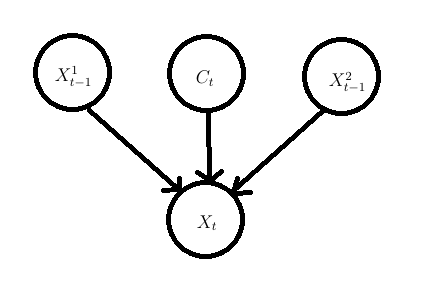
\includegraphics[width=0.5\textwidth]{Q1-3-1.png}
	
	The first state for each type of tree looks like the image below, since both states only depend on the parameters of the model.
	
	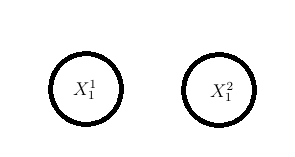
\includegraphics[width=0.5\textwidth]{Q1-3-2.png}
	
	\item[4)] $P(C_t = i | \text{parents}) = \pi$
	
	$P(X_t | C_t = i, X^1_{t-1}, X^2_{t-1}) = N(X^i_{t-1}, \sigma^2 I)$
	
	$P(X^1_1) = N(\mu_1, \sigma^2 I)$
	
	$P(X^2_1) = N(\mu_2, \sigma^2 I)$
	
	\item[5)] \textbf{TODO}
	
	$P_\theta(X^1_t, X^2_t , C_t | X_1,...,X_N) = P(C_t = i) P(X_t^{(i)} | X^{(i)}_{t-1})$
	\end{enumerate}

\item[Q2)]

	\begin{enumerate}
	\item[1)] The hidden variables are the set \{$C_t$\}. The set of observed variables are the set \{$X_t$\}.
	
	\item[2)] $\log(P_\theta(O, H)) = \log \prod_{t=1}^N P(C_t) P(X_t | X_{t-1}^1, X_{t-1}^2, C_t$)
	
	= $\sum_{t=1}^N \{ log(P(C_t)) + log(P(X_t | X_{t-1}^1, X_{t-1}^2, C_t)\}$
	
	\item[3)] \textbf{TODO}
	\end{enumerate}

\end{enumerate}

\end{document}